\documentclass[11pt,a4paper]{article}
\usepackage[no-math]{fontspec}
\usepackage{mathptmx}
\setmainfont{TeX Gyre Termes}
\usepackage{polyglossia}
\setdefaultlanguage[variant=british]{english}
\usepackage{amsmath,amssymb,bm}
\usepackage{booktabs,array,adjustbox}
\usepackage{graphicx}
\usepackage[labelfont=bf,labelsep=space,font=small,justification=centering]{caption}
\captionsetup[figure]{name=Fig.}\captionsetup[table]{name=Table}
\usepackage{lineno}
\usepackage[a4paper,margin=2.6cm]{geometry}
\usepackage{setspace}
\usepackage[authoryear,round]{natbib}
\bibpunct{(}{)}{;}{a}{}{,}
\usepackage{microtype}
\usepackage{enumitem}
\usepackage[hidelinks]{hyperref}
\usepackage{titlesec}
\usepackage[section]{placeins}
\titleformat{\section}{\normalfont\large\bfseries}{\thesection}{0.6em}{}
\titleformat{\subsection}{\normalfont\bfseries\itshape}{\thesubsection}{0.5em}{}
\titlespacing*{\section}{0pt}{2.2ex plus 1ex}{1.2ex}
\titlespacing*{\subsection}{0pt}{1.8ex plus 0.8ex}{0.8ex}
\setstretch{1.5}
\setlength{\parindent}{1.4em}
\setlength{\emergencystretch}{2em}
\renewcommand{\arraystretch}{1.08}
\setlist{nosep,leftmargin=1.6em}
\renewcommand{\floatpagefraction}{0.75}
\renewcommand{\topfraction}{0.85}
\renewcommand{\textfraction}{0.12}
\newcommand{\insR}{16.5}
\newcommand{\insY}{31.0}
\newcommand{\insGap}{$-$14.4}
\newcommand{\catR}{39.0}
\newcommand{\catY}{27.3}
\newcommand{\catGap}{11.7}
\newcommand{\catShare}{77}
\newcommand{\basR}{21.2}
\newcommand{\basY}{26.4}
\newcommand{\basGap}{$-$5.2}
\newcommand{\basShare}{10}
\newcommand{\valR}{22.9}
\newcommand{\valY}{15.9}
\newcommand{\newNat}{17.6}
\newcommand{\existNat}{7.2}
\newcommand{\cpiNat}{14.3}
\newcommand{\gapVr}{15.9}
\newcommand{\gapVrShare}{99.5}
\newcommand{\gapRaw}{13.9}
\newcommand{\gapMtwo}{16.3}
\newcommand{\aeatN}{402}
\newcommand{\aeatRent}{729}
\newcommand{\aeatRentNew}{816}
\newcommand{\aeatYld}{5.7}
\newcommand{\aeatYldNew}{6.8}
\newcommand{\aeatVr}{154,022}
\newcommand{\aeatVrNew}{145,067}
\newcommand{\gapTwoOne}{2.3}
\newcommand{\gapTwoFour}{12.7}
\newcommand{\insGapA}{$-$19.5}
\newcommand{\insGapE}{$-$7.9}
\newcommand{\bStock}{0.22}
\newcommand{\bStockAR}{[$-$0.09, 0.62]}
\newcommand{\bStockF}{21.0}
\newcommand{\bStockSe}{0.16}
\newcommand{\bGap}{0.57}
\newcommand{\bGapAR}{[0.11, 1.74]}
\newcommand{\bGapF}{11.0}
\newcommand{\bGapSe}{0.30}
\newcommand{\bGapM}{0.50}
\newcommand{\bGapMAR}{[0.06, 1.90]}
\newcommand{\bGapMF}{11.0}
\newcommand{\bGapMSe}{0.32}
\newcommand{\bGapRaw}{0.71}
\newcommand{\bGapRawAR}{[0.30, 1.73]}
\newcommand{\bGapRawF}{11.0}
\newcommand{\bGapRawSe}{0.27}
\newcommand{\bEntry}{0.83}
\newcommand{\bEntryAR}{[0.25, 2.21]}
\newcommand{\bEntryF}{11.0}
\newcommand{\bEntrySe}{0.37}
\newcommand{\bUc}{0.08}
\newcommand{\bUcAR}{[$-$0.42, 0.97]}
\newcommand{\bUcF}{16.0}
\newcommand{\bUcSe}{0.30}
\newcommand{\bPp}{$-$0.09}
\newcommand{\bPpAR}{[$-$0.60, 0.74]}
\newcommand{\bPpF}{16.0}
\newcommand{\bPpSe}{0.29}
\newcommand{\bHh}{0.89}
\newcommand{\bHhAR}{[0.34, 2.14]}
\newcommand{\bHhF}{16.0}
\newcommand{\bHhSe}{0.37}
\newcommand{\bHs}{1.26}
\newcommand{\bHsAR}{[0.69, 2.51]}
\newcommand{\bHsF}{16.0}
\newcommand{\bHsSe}{0.38}
\newcommand{\bAI}{0.18}
\newcommand{\bAIAR}{[$-$0.76, 0.81]}
\newcommand{\bAIF}{16.0}
\newcommand{\bAISe}{0.34}
\newcommand{\bAE}{0.75}
\newcommand{\bAEAR}{[$-$0.06, 1.74]}
\newcommand{\bAEF}{11.0}
\newcommand{\bAESe}{0.37}
\newcommand{\bPop}{0.82}
\newcommand{\bPopAR}{[0.17, 1.34]}
\newcommand{\bPopF}{21.0}
\newcommand{\bPopSe}{0.27}
\newcommand{\bViv}{$-$0.26}
\newcommand{\bVivAR}{[$-$0.81, 0.18]}
\newcommand{\bVivF}{21.0}
\newcommand{\bVivSe}{0.23}
\newcommand{\bPre}{$-$0.09}
\newcommand{\bPreAR}{[$-$0.31, 0.28]}
\newcommand{\bPreF}{20.9}
\newcommand{\bPreSe}{0.13}
\newcommand{\nMain}{695}
\newcommand{\nAeat}{402}
\newcommand{\rigB}{0.49}
\newcommand{\rigP}{0.019}
\newcommand{\rigSe}{0.21}
\newcommand{\rigFi}{5.9}
\newcommand{\rigBt}{0.48}
\newcommand{\rigPt}{0.003}
\newcommand{\tourInt}{$-$0.45}
\newcommand{\tourIntP}{0.025}
\newcommand{\rigEntry}{0.53}
\newcommand{\rigEntryP}{0.016}
\newcommand{\rigStock}{0.03}
\newcommand{\rigViv}{0.02}
\newcommand{\rigSea}{0.33}
\newcommand{\rigSeaP}{0.021}
\newcommand{\rigSteep}{0.78}
\newcommand{\rigSteepP}{0.066}
\newcommand{\rigAE}{0.38}
\newcommand{\rigAEP}{0.065}
\newcommand{\seasPostOne}{1.8}
\newcommand{\seasLnOne}{26}
\newcommand{\seasShareTwoThree}{6.6}
\newcommand{\seasShareTwoFive}{11.1}
\newcommand{\regLnOne}{$-$14}
\newcommand{\tRbonecovid}{$-$2.6}
\newcommand{\tNbonecovid}{$-$4.4}
\newcommand{\tRbonerecov}{1.6}
\newcommand{\tNbonerecov}{$-$8.2}
\newcommand{\tRbtwocovid}{$-$0.5}
\newcommand{\tNbtwocovid}{5.5}
\newcommand{\tRbtworecov}{3.1}
\newcommand{\tNbtworecov}{0.8}
\newcommand{\tRbthreecovid}{$-$0.8}
\newcommand{\tNbthreecovid}{6.7}
\newcommand{\tRbthreerecov}{3.1}
\newcommand{\tNbthreerecov}{$-$4.6}
\newcommand{\spCoreViv}{0.37}
\newcommand{\spCoreVivP}{0.040}
\newcommand{\spCoreR}{0.13}
\newcommand{\spCoreG}{0.29}
\newcommand{\spN}{217}
\newcommand{\spF}{48}
\newcommand{\ptiN}{276}
\newcommand{\ciStock}{0.41}
\newcommand{\ciGap}{0.43}
\newcommand{\ciGapAR}{[$-$0.03, 1.27]}
\newcommand{\ciGapRaw}{0.57}
\newcommand{\ciGapRawAR}{[0.15, 1.40]}
\newcommand{\basIv}{0.85}
\newcommand{\basIvAR}{[$-$1.42, 2.26]}
\newcommand{\basAE}{1.23}
\newcommand{\basAEAR}{[0.30, 3.10]}
\newcommand{\catIv}{$-$0.55}
\newcommand{\catIvAR}{[$-$1.25, $-$0.04]}
\newcommand{\unwGapF}{2.3}


\title{\bfseries Insiders and Outsiders in the Rental Market:\\ Entry Rents, Incomes and Housing Supply in Spain}
\author{Víctor M. Fernández-Aguilera\\[4pt]
{\small University of Almería, Almería, Spain}\\
{\small Corresponding author. E-mail: vfa084@ual.es}}
\date{}

\begin{document}
\maketitle

\begin{abstract}\noindent
Spanish tenants who stay in their homes have seen rents grow more slowly than local incomes: between 2015 and 2023, the official rent index for all leases in force rose by \insR{} log points and median income per consumption unit by \insY, and the rent-to-income ratio fell in every one of the 703 municipalities covered. Households signing a new lease faced different prices. In 2024, new leases cost \gapVr{} log points more than leases in force per euro of cadastral value, in \gapVrShare\,\% of the larger municipalities, and in Catalonia new-lease rents outpaced incomes by \catGap{} points since 2015. A stock-flow model with long leases, indexed updates and rent resets explains this insider--outsider divergence and predicts that local demand shocks load on entry rents. Using a shift-share instrument for immigration-driven population growth, I find that a cumulative inflow of 1\,\% of the population raises the quality-adjusted entry gap by \bGap\,\% and implied entry rents by \bEntry\,\%, against \bStock\,\% for all leases, while income per consumption unit does not respond and household size rises. The entry gap responds more where land is constrained by sea or slope. Tourism moves dwellings across the same entry margin, and rent caps on new leases shift contracts towards unregulated seasonal lets. Spain's rental affordability problem is a problem of access.

\medskip\noindent\textbf{Keywords} Rental housing $\cdot$ Affordability $\cdot$ Entry rents $\cdot$ Housing supply $\cdot$ Immigration $\cdot$ Spain\\
\textbf{JEL Classification} R21 $\cdot$ R31 $\cdot$ R38 $\cdot$ J61
\end{abstract}
\clearpage
\linenumbers

\section{Introduction}\label{sec:intro}

Rents top the list of economic concerns in Spain, yet the official index of rents paid by tenants has grown no faster than their incomes. Between 2015 and 2023 the INE rent index, which covers all leases declared in income-tax returns, rose by \insR{} log points; median household income per consumption unit rose by \insY. In none of the 703 municipalities with an official index did rents outpace incomes. The rent faced by a household signing a lease tells a different story. In 2024, new leases cost \gapVr{} log points more than leases in force for dwellings of the same cadastral value, and the gap is positive in \gapVrShare\,\% of the \aeatN{} municipalities with more than 20,000 inhabitants. In Catalonia, where every new lease is registered, rents on new contracts rose by \catR{} log points between 2015 and 2023, \catGap{} more than incomes.

This paper argues that the Spanish rental affordability problem is a problem of entry, explains why it arises and identifies the forces that make it larger in some markets than in others. The starting point is that the average rent of all leases, the object of official statistics, is a poor measure of the cost of finding housing today. Leases last at least five years, existing rents are updated by the consumer price index or by a legal cap, and only a small and falling share of leases is renewed each year. In such a market the adjustment to demand shocks falls on the rent reset at the start of a new contract. Incumbent tenants are insulated; households that move, form or arrive pay the market price. The affordability of insiders and the affordability of outsiders diverge.

Section~\ref{sec:theory} formalises this idea in a stock-flow model of a local rental market with contract duration, indexed updates and rent resets, in which the incomes and the size of households respond to the same shocks. The model delivers three predictions. A demand shock raises entry rents more than the average rent of all leases, and more where supply is inelastic. Whether it worsens affordability depends on whether it raises the income of those who enter, which a measure of income per household can conceal when households grow larger. Rules that protect incumbents widen the gap between entry rents and the rents of sitting tenants, while caps on entry rents narrow it at the cost of fewer new leases.

The empirical analysis tests these predictions with open administrative data. Tax statistics give, for 2024, the rent, floor area and cadastral value of new leases and of all leases in every municipality above 20,000 inhabitants, which allows a quality-adjusted measure of the entry gap. Deposit registers in Catalonia, the Basque Country and the Comunitat Valenciana record rents at signature. The household income atlas gives income per consumption unit and household size by municipality. The demand shock is the immigration-driven inflow of residents predicted by a shift-share instrument based on the settlement of 33 origin groups in 2003 and their national growth \citep{saiz2007,goldsmith2020,borusyak2022}, taken from a companion paper \citep{fernandez2026}.

Five results stand out. First, a cumulative inflow of 1\,\% of the population raises the quality-adjusted entry gap by \bGap\,\% (Anderson-Rubin set \bGapAR) and implied entry rents by \bEntry\,\% \bEntryAR, while the effect on the rent of all leases is \bStock{} and not significant. Second, the same shock does not raise income per consumption unit (\bUc), but it raises household size (\bHs) and therefore income per household (\bHh): measured per household, affordability would appear to improve because more adults share each dwelling. Third, the dwelling stock does not respond, and the entry gap responds more to demand where land is constrained by sea or steep slopes (\rigB{} per standard deviation, $p$ = \rigP). Fourth, tourism moves dwellings across the same entry margin: when tourism collapsed in 2020--21, more long-term leases were signed in municipalities where more than 3\,\% of dwellings were tourist lets, and rents on new leases rose by about 3\,\% with the recovery. Fifth, the Catalan cap on new-contract rents lowered entry rents and the number of leases and raised the share of unregulated seasonal leases by \seasPostOne{} percentage points.

The paper contributes to three literatures. It adds to the economics of rental affordability \citep{quigley2004,khametshin2024} a distinction between insiders and outsiders and evidence that the two diverge. It contributes to the measurement of rents by showing why indices of all leases \citep{genesove2003,ambrose2015} understate what entrants pay, and by constructing a quality-adjusted entry gap from tax data. And it links the literatures on local demand shocks and supply constraints \citep{saiz2010,glaeser2018,hilber2016} and on rent regulation \citep{autor2014,diamond2019,jofre2023} through the margin at which adjustment takes place.

\section{Institutions and measurement}\label{sec:institutions}

\textit{Leases and updates.} Since March 2019 residential leases in Spain last at least five years when the landlord is a natural person and seven when it is a company, and annual updates of existing leases are usually tied to the consumer price index. Updates were capped at 2\,\% from the end of March 2022 to the end of 2023 and at 3\,\% in 2024, and since 2025 they follow a reference index published by INE. Rents are set freely at the start of a new lease except in markets declared tensioned under the 2023 Housing Act, where they are capped by the rent of the previous lease and a reference index; Catalonia applied this cap in 140 municipalities from 16 March 2024 and in 131 more from October 2024.

\textit{Measuring rents.} The INE index (IPVA) averages the rents of all leases in force declared in income-tax returns, excluding the Basque Country and Navarre. Since 2021 INE also publishes separate indices for new and existing leases, with weights: new leases accounted for 17.6\,\% of the index in 2021 and 12.3\,\% in 2024. The tax agency publishes, for 2024, the average rent, floor area and cadastral reference value of all leases and of leases signed in the year, by municipality above 20,000 inhabitants. Deposit registers record leases at signature in Catalonia (mean rent, municipality and quarter, since 2005), the Basque Country (rent per m$^2$ built, municipality and year, since 2016) and the Comunitat Valenciana (deposit amount, since 2020).

\section{Related literature}\label{sec:lit}

Rental affordability is usually measured as the ratio of rent to the income of renters \citep{quigley2004}. For Spain, \citet{khametshin2024} document the rise in rental demand since 2015 among young and foreign-born households and in large urban and tourist areas, and the high rent burden of low-income tenants, and describe the quantification of its causes as an open question. Indices of rents on all leases move slowly because existing rents are sticky \citep{genesove2003} and because tenants who stay pay less than new ones \citep{ambrose2015}. Rent control turns that wedge into a policy instrument: it benefits incumbent tenants and reduces the supply of rental housing to newcomers \citep{autor2014,diamond2019,kholodilin2024}, and in Catalonia it lowered rents and the number of leases signed \citep{jofre2023,perez2026}.

Local demand shocks are capitalised into rents where supply is inelastic \citep{roback1982,saiz2010,glaeser2018,hilber2016,hsieh2019}. Immigration is the standard source of such shocks: \citet{saiz2007} finds that an inflow of 1\,\% of a city's population raises rents by about 1\,\%, and \citet{gonzalez2013} and \citet{sanchis2023} study house prices in Spain. Short-term rentals reallocate dwellings from residents to visitors \citep{barron2021}; in Barcelona they raised rents \citep{garcialopez2020}, and in Lisbon the collapse of tourism in 2020 lowered rents and increased the long-term rental supply \citep{batalha2022}. None of these strands separates the rents paid by insiders from those faced by entrants, which is the focus of this paper.

\section{A model of insiders, entrants and rent resets}\label{sec:theory}

\subsection{Leases, resets and the index of all leases}

A local market $i$ has a stock of rental dwellings let on long leases. In year $t$ a share $\lambda_{it}$ of leases ends and the dwelling is relet at the market-clearing entry rent $R^*_{it}$; the remaining leases are updated by $u_t=\min(\pi_t,\bar u_t)$, inflation or a legal cap. The log of the average rent of all leases, $\bar r_{it}$, then satisfies
\begin{equation}\label{eq:index}
\bar r_{it}=\lambda_{it}\,r^*_{it}+(1-\lambda_{it})\,(\bar r_{i,t-1}+u_t),
\end{equation}
and the entry gap $G_{it}\equiv r^*_{it}-\bar r_{it}$ evolves as
\begin{equation}\label{eq:gap}
G_{it}=(1-\lambda_{it})\,\big[G_{i,t-1}+\Delta r^*_{it}-u_t\big].
\end{equation}
The gap widens whenever entry rents grow faster than the update rule, and it is more persistent the lower the turnover $\lambda$. Longer minimum durations lower $\lambda$; caps on updates lower $u_t$. Both widen the gap for a given path of entry rents. A cap on entry rents limits $\Delta r^*$ directly.

\subsection{Entry rents, incomes and household size}

Entry rents clear the flow market for new leases. Demand comes from households that form, move or arrive; their number grows with the local population $N_{it}$, and each consumes $q_{it}=A\,(Y_{it}/S_{it})^{\alpha}\,R_{it}^{*\,-\eta}$ units of housing per person, where $Y_{it}/S_{it}$ is income per consumption unit, $S_{it}$ an equivalence scale that increases with household size, and $\eta$ the price elasticity of space per person. A high $\eta$ means that higher rents are absorbed by sharing dwellings. Supply comes from dwellings released by sitting tenants, new construction with elasticity $\sigma_i$, and dwellings reallocated from tourist use or non-use with elasticity $\varepsilon_i$. Log-linearising, a population shock $d\ln N_{it}$ raises entry rents by
\begin{equation}\label{eq:entry}
d\,r^*_{it}=\frac{d\ln N_{it}+\alpha\,(d\ln Y_{it}-d\ln S_{it})}{\eta+\varepsilon_i+\sigma_i},
\end{equation}
and the affordability of entrants, $A^E_{it}=r^*_{it}-\ln(Y_{it}/S_{it})$, changes by
\begin{equation}\label{eq:aff}
dA^E_{it}=d\,r^*_{it}-\big(d\ln Y_{it}-d\ln S_{it}\big).
\end{equation}
The model yields three predictions.

\begin{description}
\item[P1 (entry loading).] A demand shock raises entry rents by more than the rent of all leases, by a factor of the order of $1/\lambda$ in the short run, so that the entry gap $G$ widens.
\item[P2 (income measurement).] A shock that raises household size $S$ raises income per household mechanically without raising income per consumption unit. Affordability measured per household can improve while the affordability of entrants deteriorates.
\item[P3 (amplification).] The response of entry rents is larger where new supply ($\sigma_i$) and reallocation ($\varepsilon_i$) are less elastic: in land-constrained markets and where few dwellings can be moved from other uses into long-term letting.
\end{description}

Tourism enters as a shift in $\varepsilon_i$: tourist demand withdraws dwellings from long-term letting, and a collapse in tourist demand returns them, so its effects appear in entry rents and in the number of new leases. Rent caps on new leases lower measured $r^*$ but reduce the number of leases signed if owners move dwellings to unregulated uses, such as seasonal lets.

\section{Data}\label{sec:data}

\textit{Entry gap.} The main outcome is the quality-adjusted entry gap in 2024 from the tax statistics of dwellings declared in income-tax returns:
\[
G^{VR}_i=\ln\!\Big(\frac{\text{rent}^{new}_i}{\text{value}^{new}_i}\Big)-\ln\!\Big(\frac{\text{rent}^{all}_i}{\text{value}^{all}_i}\Big),
\]
where value is the mean cadastral reference value of the dwellings. $G^{VR}$ equals the log ratio of gross yields on new and on all leases. A version per m$^2$ and the raw gap are used for robustness. In Spain as a whole, new leases averaged \aeatRentNew{} euros per month against \aeatRent{} for all leases, while new leases were on dwellings of lower value (\aeatVrNew{} against \aeatVr{} euros): the gross yield was \aeatYldNew\,\% against \aeatYld\,\%.

\textit{Rents and incomes over time.} INE indices for all, new and existing leases; deposit registers in Catalonia, the Basque Country and the Comunitat Valenciana; and the INE household income atlas (2015--2023) for median net income per consumption unit, income per person and per household, and average household size.

\textit{Demand shock and controls.} The cumulative net inflow of foreign-born residents between 2015 and 2024 relative to 2015 population, from the municipal register (to 2021) and the annual census (from 2021), using within-source changes. The instrument sums the companion paper's annual shift-share predictions over the same years. Controls are predetermined characteristics from the 2011 census and 2012 firm counts.

\textit{Supply constraints, tourism, regulation and tenure.}
\begin{itemize}
\item Supply constraints: share of land within 10 km of each municipality that is sea or has a slope above 15\,\%, computed from the Copernicus 90-metre digital elevation model in the spirit of \citet{saiz2010}. Cadastral dwelling counts measure the supply response.
\item Tourism: tourist dwellings as a share of all dwellings (INE, August 2020).
\item Regulation: seasonal leases by municipality and quarter in Catalonia (2023--2026).
\item Tenure: appraised housing values by municipality (Ministry of Housing) relative to income, as a measure of exposure to the rise in mortgage rates.
\end{itemize}
All data are public and are downloaded by the replication code.

\section{Insiders and entrants}\label{sec:facts}

Table~\ref{tab:facts} and figure~\ref{fig:facts} set out the central facts. For all leases, rents grew by \insR{} log points between 2015 and 2023 and income per consumption unit by \insY: the rent-to-income ratio of sitting tenants fell by \insGap{} points on average, by \insGapA{} in municipalities of 10,000--20,000 inhabitants and by \insGapE{} in the largest cities. Not a single municipality shows the opposite. New leases tell a different story in two of the three regions with registers. In Catalonia, rents on new leases rose by \catR{} log points against \catY{} for incomes, and they outpaced incomes in \catShare\,\% of municipalities. The gap between entry rents and incomes increases with the size of the municipality (figure~\ref{fig:facts}b). In the Comunitat Valenciana, deposits on new leases rose by \valR{} points between 2020 and 2023, against \valY{} for incomes. In the Basque Country, however, rents per m$^2$ on new leases rose by \basR{} points between 2016 and 2023, less than incomes (\basY), and they outpaced incomes in only \basShare\,\% of municipalities: the divergence at entry is not universal.

\begin{figure}[!htbp]\centering
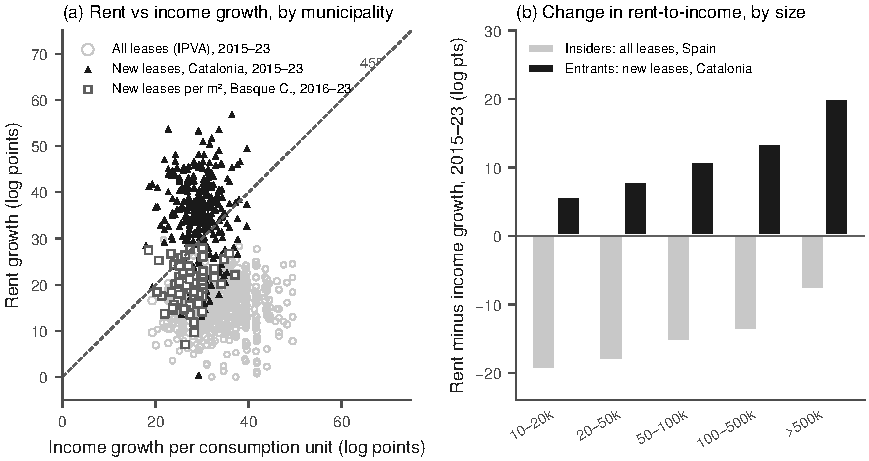
\includegraphics[width=\linewidth]{fig/fig1_insiders_entrants.pdf}
\caption{Rents of insiders and entrants against incomes}\label{fig:facts}
\begin{minipage}{0.95\linewidth}\footnotesize\vspace{2pt}
\textit{Notes}: panel (a), growth of rents and of median income per consumption unit by municipality: index of all leases (IPVA, 2015--2023), mean rent of new leases in Catalonia (2015--2023, municipalities with at least 30 leases in 2015) and rent per m$^2$ of new leases in the Basque Country (2016--2023). Panel (b), population-weighted difference between rent and income growth by size of municipality. Sources: INE, Generalitat de Catalunya, Gobierno Vasco.
\end{minipage}
\end{figure}

\begin{table}[!htbp]\centering\small
\caption{Rents of insiders and entrants against incomes}\label{tab:facts}
\begin{adjustbox}{max width=\linewidth}\begin{tabular}{lllcccc}\toprule
Rent measure & Period & Units & Rent growth & Income growth & Difference & Share with rent $>$ income\\
 & & & \multicolumn{3}{c}{(log points, weighted)} & \\\midrule
All leases (IPVA), Spain & 2015--2023 & 703 municipalities & 1650.0 & 31.0 & 1619.0 & 0\,\%\\
New leases (deposits), Catalonia & 2015--2023 & 289 municipalities & 39.0 & 27.3 & 11.7 & 77\,\%\\
New leases per m$^2$ (deposits), Basque Country & 2016--2023 & 67 municipalities & 21.2 & 26.4 & $-$5.2 & 10\,\%\\
Deposits on new leases, Comunitat Valenciana & 2020--2023 & 104 municipalities & 22.9 & 15.9 & 7.0 & --\\
\addlinespace
\multicolumn{7}{l}{\textit{Entry gap: new leases relative to leases in force}}\\
INE index, new vs existing, Spain & 2021--2024 & national & 17.6 & 7.2 & 10.4 & \\
AEAT, new vs all leases, per euro of cadastral value & 2024 & 402 municipalities & & & 15.9 & 99.5\,\%$^a$\\
\bottomrule\end{tabular}\end{adjustbox}
\begin{minipage}{0.97\linewidth}\footnotesize\vspace{4pt}
\textit{Notes}: income is the median net income per consumption unit of the municipality (INE household income atlas). Means weighted by 2015 population. IPVA: index of all leases in force (tax returns). Deposit registers record leases at signature: mean rent in Catalonia (contracts of more than one year), rent per m$^2$ built in the Basque Country (free-market collective main residences), deposit amount in the Comunitat Valenciana (one month of rent by law; partial coverage). AEAT: tax statistics of dwellings declared in 2024, municipalities above 20,000 inhabitants; the entry gap is $\ln(\text{rent}_{new}/\text{value}_{new})-\ln(\text{rent}_{all}/\text{value}_{all})$. $^a$ Share of municipalities with a positive gap.
\end{minipage}\end{table}

The entry gap is widening nationally. Relative to 2015, the INE index of new leases exceeded the index of existing leases by \gapTwoOne{} log points in 2021 and by \gapTwoFour{} in 2024, and the gap widened in every province (figure~\ref{fig:gap}a). In levels, the tax data show a quality-adjusted gap of \gapVr{} log points in 2024, with a median of about 15 points in every size class (figure~\ref{fig:gap}b). New leases are signed on dwellings of lower value and similar size; the raw gap (\gapRaw) understates the quality-adjusted one.

\begin{figure}[!htbp]\centering
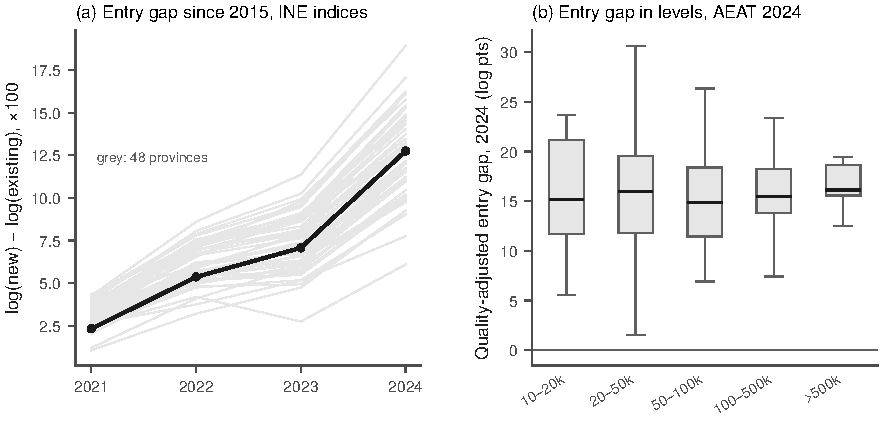
\includegraphics[width=\linewidth]{fig/fig2_entry_gap.pdf}
\caption{The entry gap over time and in levels}\label{fig:gap}
\begin{minipage}{0.95\linewidth}\footnotesize\vspace{2pt}
\textit{Notes}: panel (a), $100\times\ln(\text{index}_{new}/\text{index}_{existing})$, both indices with base 2015 = 100 (INE table 59005), Spain and 48 provinces. Panel (b), quality-adjusted entry gap in 2024 (AEAT) by size of municipality: median, interquartile range and 1.5 interquartile-range whiskers.
\end{minipage}
\end{figure}

\section{Empirical strategy}\label{sec:strategy}

For municipality $i$ in province $p$,
\begin{equation}\label{eq:est}
y_i=\beta\, x_i+\bm{w}_i'\bm\gamma+\delta_p+\varepsilon_i,
\end{equation}
where $x_i$ is the cumulative foreign-born inflow relative to 2015 population and $y_i$ is, in turn, the entry gap, the growth of the rent of all leases, implied entry-rent growth (the sum of the two), income per consumption unit, income per person and per household, household size, population and the dwelling stock. Affordability outcomes are rent growth minus growth of income per consumption unit, for insiders (all leases) and for entrants (implied entry rents). $x_i$ is instrumented with the cumulative shift-share prediction $z_i=\sum_t\sum_o \ell_{io}\,(g_{ot}-g_{opt})/P_i$, where $\ell_{io}$ is municipality $i$'s share of the 2003 national stock of origin $o$ and $g_{ot}-g_{opt}$ the national change in that stock excluding province $p$. Identification follows \citet{borusyak2022}: the national, leave-province-out growth of each origin group is assumed to be as good as random with respect to local trends in rents, conditional on province fixed effects and predetermined characteristics. Regressions are weighted by 2015 population, standard errors are clustered by province and Anderson-Rubin sets are reported throughout. The pre-period falsification regresses rent growth in 2012--2015 on the 2015--2024 inflow.

Prediction P3 is tested by interacting the inflow with standardised measures of geographic constraints and instrumenting the interaction with $z_i$ times the constraint. Geographic constraints are predetermined and, unlike density or construction, do not reflect past demand.

\section{Results}\label{sec:results}

\subsection{Where a demand shock goes}

Table~\ref{tab:main} and figure~\ref{fig:shock} report the effects of the demand shock. A cumulative inflow of 1\,\% of the population raises the quality-adjusted entry gap by \bGap\,\% (Anderson-Rubin set \bGapAR; first-stage $F$ \bGapF), the gap per m$^2$ by \bGapM\,\% and the raw gap by \bGapRaw\,\%. Combined with the response of the rent of all leases, \bStock\,\% \bStockAR, the implied response of entry rents is \bEntry\,\% \bEntryAR: entry rents respond several times more than the average rent of all leases, as prediction P1 implies.

The shock raises population by \bPop\,\% per point of inflow: immigrants do not displace natives on net. It does not raise income per consumption unit (\bUc, \bUcAR) or income per person (\bPp). It raises household size by \bHs\,\% \bHsAR{} and income per household by \bHh\,\% \bHhAR. Prediction P2 holds: households absorb the shock partly by sharing dwellings, which raises household income without raising the income available per person. The affordability of entrants deteriorates by \bAE\,\% per point of inflow \bAEAR, while that of insiders does not change significantly (\bAI). The dwelling stock does not respond (\bViv, \bVivAR), and the falsification test passes: the inflow of 2015--2024 does not predict rent growth in 2012--2015 (\bPre, \bPreAR).

\begin{figure}[!htbp]\centering
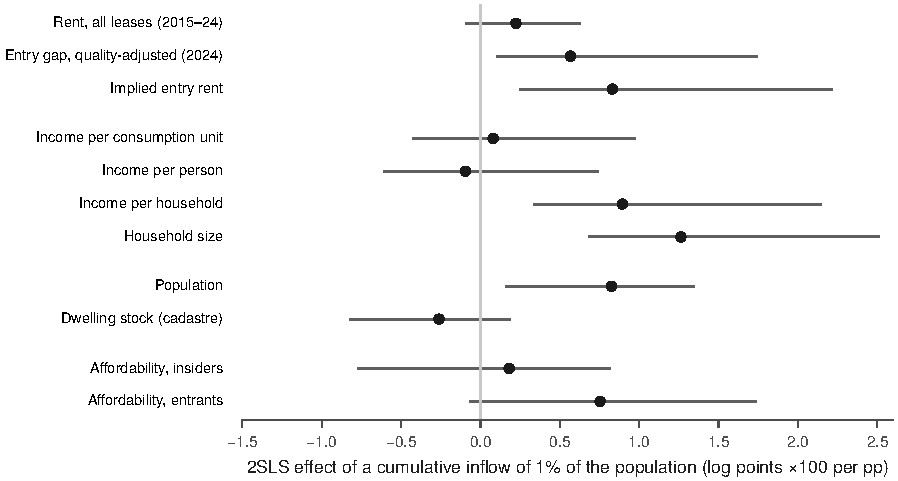
\includegraphics[width=0.9\linewidth]{fig/fig3_where_shock_goes.pdf}
\caption{Where a local demand shock goes}\label{fig:shock}
\begin{minipage}{0.88\linewidth}\footnotesize\vspace{2pt}
\textit{Notes}: 2SLS coefficients of table~\ref{tab:main} and Anderson-Rubin 95\,\% sets; arrows mark sets that extend beyond the axis.
\end{minipage}
\end{figure}

\begin{table}[!htbp]\centering\small
\caption{Where a local demand shock goes: rents, entry rents, incomes and households}\label{tab:main}
\begin{adjustbox}{max width=\linewidth}\begin{tabular}{lcccccc}\toprule
Outcome & 2SLS & SE & AR 95\% set & First-stage $F$ & $N$ & Mean\\\midrule
\multicolumn{7}{l}{\textit{A. Rents}}\\
Rent, all leases, 2015--2024 & 0.22 & (0.16) & [$-$0.09, 0.62] & 21.0 & 695 & 0.200\\
Entry gap, per euro of cadastral value, 2024 & 0.57 & (0.30) & [0.11, 1.74] & 11.0 & 402 & 0.159\\
Entry gap, per m$^2$, 2024 & 0.50 & (0.32) & [0.06, 1.90] & 11.0 & 402 & 0.163\\
Entry gap, raw, 2024 & 0.71 & (0.27) & [0.30, 1.73] & 11.0 & 402 & 0.139\\
Implied entry rent (all leases + quality-adjusted gap) & 0.83 & (0.37) & [0.25, 2.21] & 11.0 & 402 & 0.363\\
\multicolumn{7}{l}{\textit{B. Incomes and households, 2015--2023}}\\
Income per consumption unit (median) & 0.08 & (0.30) & [$-$0.42, 0.97] & 16.0 & 695 & 0.310\\
Income per person & $-$0.09 & (0.29) & [$-$0.60, 0.74] & 16.0 & 695 & 0.318\\
Income per household & 0.89 & (0.37) & [0.34, 2.14] & 16.0 & 695 & 0.293\\
Household size & 1.26 & (0.38) & [0.69, 2.51] & 16.0 & 695 & $-$0.022\\
\multicolumn{7}{l}{\textit{C. Affordability}}\\
Insiders: rent of all leases minus income per consumption unit & 0.18 & (0.34) & [$-$0.76, 0.81] & 16.0 & 695 & $-$0.144\\
Entrants: implied entry rent minus income per consumption unit & 0.75 & (0.37) & [$-$0.06, 1.74] & 11.0 & 402 & 0.057\\
\multicolumn{7}{l}{\textit{D. Quantities and falsification}}\\
Population & 0.82 & (0.27) & [0.17, 1.34] & 21.0 & 695 & 0.065\\
Dwelling stock (cadastre) & $-$0.26 & (0.23) & [$-$0.81, 0.18] & 21.0 & 695 & 0.038\\
Rent of all leases, 2012--2015 (pre-period) & $-$0.09 & (0.13) & [$-$0.31, 0.28] & 20.9 & 694 & $-$0.035\\
\bottomrule\end{tabular}\end{adjustbox}
\begin{minipage}{0.97\linewidth}\footnotesize\vspace{4pt}
\textit{Notes}: one observation per municipality. Treatment: cumulative net foreign-born inflow between 1 January 2015 and 1 January 2025 (2024 for panels B and C, insiders) relative to 2015 population, instrumented with the corresponding sum of leave-own-province-out shift-share predictions (33 origins, 2003 settlement). All regressions include province fixed effects and predetermined controls (2011 census: log population, renting, vacancy, tertiary education, share aged 65+; 2012: construction, industry and trade-hospitality shares of firms, firms per capita; coastal and FUA-core indicators), population weights and standard errors clustered by province. Entry-gap outcomes are available for the municipalities above 20,000 inhabitants in the AEAT statistics. AR: Anderson-Rubin set.
\end{minipage}\end{table}

\subsection{Supply constraints}

Table~\ref{tab:rigidity} and figure~\ref{fig:rigidity} test prediction P3. A one-standard-deviation increase in the share of undevelopable land within 10 km raises the effect of the demand shock on the entry gap by \rigB{} ($p$ = \rigP) and on implied entry rents by \rigEntry{} ($p$ = \rigEntryP). The interaction is similar for the sea (\rigSea, $p$ = \rigSeaP) and for steep slopes (\rigSteep, $p$ = \rigSteepP), and it survives the inclusion of the interaction between the inflow and tourist exposure (\rigBt, $p$ = \rigPt). The geographic constraint does not change the response of the rent of all leases (\rigStock) or of the cadastral dwelling stock (\rigViv), which is close to zero everywhere. The amplification works through the entry margin, not through measured construction. Two caveats apply: the partial first-stage $F$ of the interaction is modest (\rigFi{} for the composite measure), and the marginal effect on the entry gap is only clearly positive above about 60\,\% of undevelopable land.

\begin{figure}[!htbp]\centering
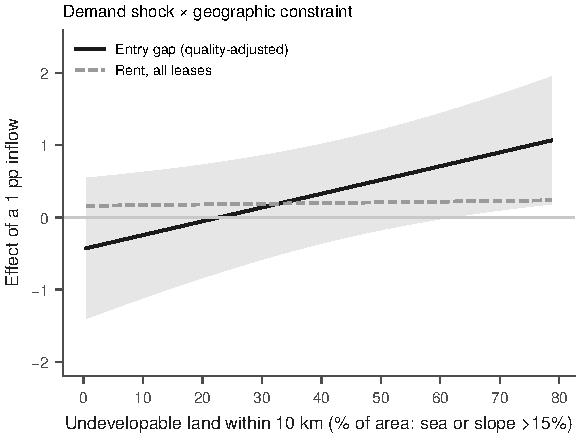
\includegraphics[width=0.62\linewidth]{fig/fig4_rigidity.pdf}
\caption{Demand shocks and geographic constraints}\label{fig:rigidity}
\begin{minipage}{0.75\linewidth}\footnotesize\vspace{2pt}
\textit{Notes}: marginal effect of a 1\,pp inflow on the quality-adjusted entry gap and on the rent of all leases as a function of undevelopable land within 10 km (5th to 95th percentile), from table~\ref{tab:rigidity}; 95\,\% band for the entry gap.
\end{minipage}
\end{figure}

\begin{table}[!htbp]\centering\small
\caption{Demand shocks and geographic constraints on supply}\label{tab:rigidity}
\begin{adjustbox}{max width=\linewidth}\begin{tabular}{llcccccc}\toprule
Outcome & Constraint & Inflow & Inflow $\times$ constraint & $p$ & $F$ (inflow; interaction) & \multicolumn{2}{c}{Net of inflow $\times$ tourism}\\\cmidrule(lr){7-8}
 & & & & & & Inflow $\times$ constraint & Inflow $\times$ tourism\\\midrule
Entry gap (quality-adjusted) & Undevelopable & 0.12 (0.37) & 0.49** (0.21) & 0.019 & 10.6; 5.9 & 0.48*** (0.17) & $-$0.45** (0.20)\\
 & Sea & $-$0.02 (0.31) & 0.33** (0.14) & 0.021 & 26.4; 11.5 & 0.43*** (0.13) & $-$0.46** (0.19)\\
 & Slope $>$15\% & 0.76 (0.50) & 0.78* (0.42) & 0.066 & 10.6; 9.5 & 0.60** (0.29) & $-$0.40 (0.29)\\
\addlinespace
Implied entry rent & Undevelopable & 0.34 (0.34) & 0.53** (0.22) & 0.016 & 10.6; 5.9 & 0.51*** (0.19) & $-$0.37** (0.17)\\
 & Sea & 0.19 (0.28) & 0.36** (0.17) & 0.029 & 26.4; 11.5 & 0.45*** (0.12) & $-$0.38** (0.15)\\
 & Slope $>$15\% & 0.99 (0.53) & 0.78* (0.41) & 0.056 & 10.6; 9.5 & 0.58* (0.31) & $-$0.33 (0.27)\\
\addlinespace
Entrants' affordability & Undevelopable & 0.40 (0.30) & 0.38* (0.21) & 0.065 & 10.6; 5.9 & 0.33 (0.23) & 0.08 (0.18)\\
 & Sea & 0.19 (0.29) & 0.33* (0.19) & 0.078 & 26.4; 11.5 & 0.30* (0.17) & 0.08 (0.19)\\
 & Slope $>$15\% & 0.84 (0.48) & 0.52 (0.37) & 0.165 & 10.6; 9.5 & 0.45 (0.39) & 0.09 (0.24)\\
\addlinespace
Rent, all leases & Undevelopable & 0.19 (0.14) & 0.03 (0.11) & 0.814 & 16.1; 8.2 & & \\
 & Sea & 0.22 (0.11) & 0.00 (0.05) & 0.929 & 51.7; 16.5 & & \\
 & Slope $>$15\% & 0.19 (0.18) & 0.00 (0.16) & 0.981 & 15.0; 12.5 & & \\
\addlinespace
Dwelling stock & Undevelopable & $-$0.31 (0.25) & 0.02 (0.09) & 0.800 & 16.1; 8.2 & & \\
 & Sea & $-$0.28 (0.29) & 0.02 (0.07) & 0.746 & 51.7; 16.5 & & \\
 & Slope $>$15\% & $-$0.32 (0.24) & 0.00 (0.13) & 0.997 & 15.0; 12.5 & & \\
\addlinespace
\bottomrule\end{tabular}\end{adjustbox}
\begin{minipage}{0.97\linewidth}\footnotesize\vspace{4pt}
\textit{Notes}: 2SLS with two endogenous regressors, the inflow and its interaction with a standardised constraint, instrumented with the shift-share prediction and its interaction. Constraints: share of land within 10 km of the municipality centroid that is sea or has slope above 15\,\% (Copernicus DEM GLO-90), and each component. Same fixed effects, controls, weights and clustering as table~\ref{tab:main}. $F$: first-stage partial $F$ statistics. The last two columns add the inflow interacted with the share of dwellings in tourist use (2020) and its instrument. *** $p<0.01$, ** $p<0.05$, * $p<0.1$.
\end{minipage}\end{table}

\subsection{Tourism}

The interaction between the inflow and tourist exposure in table~\ref{tab:rigidity} is negative (\tourInt, $p$ = \tourIntP): the same demand shock widens the entry gap less where many dwellings are tourist lets, as if part of that stock acted as a reserve for long-term letting. The collapse of tourism in 2020--21 tests this margin directly (table~\ref{tab:channels}, panel A; figure~\ref{fig:tourism}). In Catalan municipalities where 3--8\,\% and more than 8\,\% of dwellings were tourist lets, the number of new long-term leases rose by \tNbtwocovid\,\% and \tNbthreecovid\,\% during the collapse relative to municipalities with little tourist letting. With the recovery, rents on new leases rose by about 3\,\% in the same groups (\tRbtworecov\,\% and \tRbthreerecov\,\%). Below 3\,\% of dwellings there is no reallocation of leases. The pattern points to a threshold: tourism shapes entry rents where tourist lets are a sizable share of the stock.

\begin{figure}[!htbp]\centering
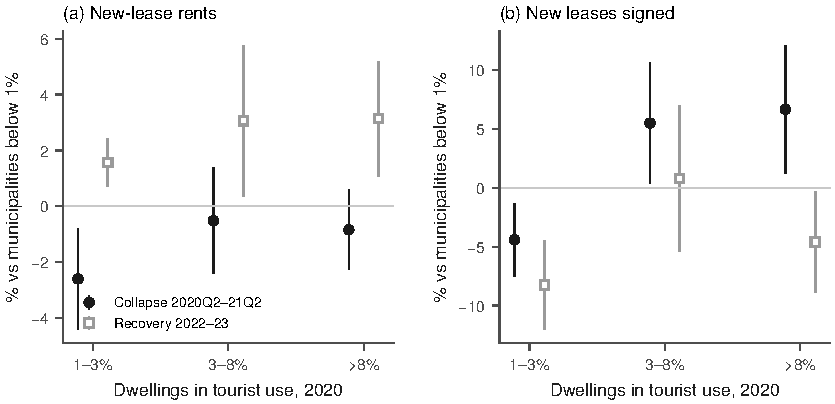
\includegraphics[width=0.95\linewidth]{fig/fig5_tourism_threshold.pdf}
\caption{Tourist dwellings and new leases during the collapse and recovery of tourism}\label{fig:tourism}
\begin{minipage}{0.92\linewidth}\footnotesize\vspace{2pt}
\textit{Notes}: coefficients and 95\,\% intervals of table~\ref{tab:channels}, panel A, by share of dwellings in tourist use in August 2020.
\end{minipage}
\end{figure}

\subsection{Regulation}

Prediction~\eqref{eq:gap} implies that caps on updates widen the entry gap and that caps on entry rents narrow it. Between 2021 and 2024 the national entry gap widened in every year, most in 2024, when new-lease rents rose by 8.8\,\% and existing leases by 2.8\,\%; the update caps of 2022--2024 held the index of all leases below inflation. The Catalan cap on new leases, evaluated in the companion analysis with stacked difference-in-differences, lowered new-lease rents by about 5\,\% and the number of new leases by about 18\,\% in the first wave. Table~\ref{tab:channels}, panel B, shows where part of those leases went: after the cap, the share of seasonal leases among new leases rose by \seasPostOne{} percentage points in the first wave (seasonal leases are exempt from the cap) and seasonal leases rose by about \seasLnOne\,\%. In the whole sample their share rose from \seasShareTwoThree\,\% in 2023 to \seasShareTwoFive\,\% in 2025. The register of seasonal leases begins in 2023, so the pre-period is short (figure~\ref{fig:cap}).

\begin{figure}[!htbp]\centering
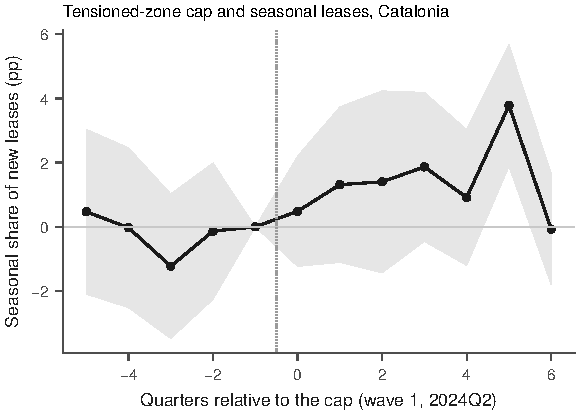
\includegraphics[width=0.62\linewidth]{fig/fig6_cap_seasonal.pdf}
\caption{Tensioned-zone cap and seasonal leases}\label{fig:cap}
\begin{minipage}{0.75\linewidth}\footnotesize\vspace{2pt}
\textit{Notes}: event study of the seasonal share of new leases in the first wave of designated municipalities relative to never-designated ones, 2023Q1--2025Q4; 95\,\% band; clusters by municipality.
\end{minipage}
\end{figure}

\subsection{Tenure and spillovers}

If the rise in mortgage rates from 2022 had pushed would-be buyers into renting, rents should have risen more where housing was most expensive relative to incomes. Table~\ref{tab:channels}, panel C, finds no break after 2022 in the index of all leases, and no association between price-to-income and the entry gap in 2024; the tenure channel is not supported by these data. Panel D studies spillovers within functional urban areas: the demand shock of the core city raises the dwelling stock of its peripheral municipalities (\spCoreViv, $p$ = \spCoreVivP) but has small and imprecise effects on their rents and entry gaps. Supply in the periphery responds to demand in the core; rents there do not measurably follow.

\begin{table}[!htbp]\centering\small
\caption{Tourism, regulation, tenure and spillovers}\label{tab:channels}
\begin{adjustbox}{max width=\linewidth}\begin{tabular}{lcccccc}\toprule
\multicolumn{7}{l}{\textit{A. Tourist dwellings and new leases, Catalonia (\% relative to municipalities with $<$1\,\% of dwellings in tourist use)}}\\
Exposure in 2020 & \multicolumn{3}{c}{New-lease rents} & \multicolumn{3}{c}{New leases signed}\\\cmidrule(lr){2-4}\cmidrule(lr){5-7}
 & Collapse & Recovery & 2024--25 & Collapse & Recovery & 2024--25\\
1--3\,\% & $-$2.6*** & 1.6*** & $-$0.9 & $-$4.4*** & $-$8.2*** & $-$12.4***\\
3--8\,\% & $-$0.5 & 3.1** & 3.3*** & 5.5** & 0.8 & 9.8\\
$>$8\,\% & $-$0.8 & 3.1*** & 2.3* & 6.7** & $-$4.6** & 8.8**\\
\midrule
\multicolumn{7}{l}{\textit{B. Tensioned-zone cap and seasonal leases, Catalonia, 2023Q1--2025Q4 (DiD)}}\\
 & \multicolumn{2}{c}{Seasonal share (pp)} & \multicolumn{2}{c}{log seasonal leases} & \multicolumn{2}{c}{log regular leases}\\
Wave 1 (2024Q2) & \multicolumn{2}{c}{1.82*** (0.39)} & \multicolumn{2}{c}{0.26*** (0.04)} & \multicolumn{2}{c}{$-$0.14*** (0.03)}\\
Wave 2 (2024Q4) & \multicolumn{2}{c}{0.94** (0.40)} & \multicolumn{2}{c}{0.09*** (0.03)} & \multicolumn{2}{c}{$-$0.08*** (0.03)}\\
\midrule
\multicolumn{7}{l}{\textit{C. Tenure: price-to-income in 2021 (s.d.) $\times$ year, rent of all leases (reference 2021)}}\\
2019 & 2020 & 2022 & 2023 & 2024 & Entry gap 2024 & \\
0.82*** & 0.21** & 0.06 & 0.07 & $-$0.01 & $-$0.01 & \\
\midrule
\multicolumn{7}{l}{\textit{D. Spillovers: shift-share shock of the core city on peripheral municipalities of the same FUA (reduced form)}}\\
 & Rent, all leases & Entry gap & Population & Inflow & Dwellings & \\
Own shock & $-$0.04 & 0.13 & $-$0.32** & $-$0.00 & $-$0.20* & \\
Core shock & 0.13 & 0.29 & 0.39 & 0.03 & 0.37** & \\
\bottomrule\end{tabular}\end{adjustbox}
\begin{minipage}{0.97\linewidth}\footnotesize\vspace{4pt}
\textit{Notes}: panel A, Catalan municipalities with new leases in every quarter of 2019; municipality and quarter fixed effects and exposure-bin $\times$ calendar-quarter terms; collapse 2020Q2--2021Q2, recovery 2022--2023; population weights; clusters by municipality. Panel B: municipality and quarter fixed effects and tourist exposure $\times$ calendar quarter; clusters by municipality; the seasonal-lease register starts in 2023. Panel C: IPVA municipalities with an appraised value (MIVAU, municipalities above 25,000 inhabitants); municipality and province $\times$ year fixed effects and predetermined characteristics $\times$ year; coefficients $\times$100. Panel D: 217 peripheral municipalities in 48 functional urban areas; province fixed effects and controls; clusters by FUA. *** $p<0.01$, ** $p<0.05$, * $p<0.1$.
\end{minipage}\end{table}

\section{Robustness}\label{sec:robust}

Table~\ref{tab:robust} reports alternative instruments, weights and registers. With the companion paper's instrument, which sums annual predictions with centred timing over the 699 municipalities of its sample, the effect on the rent of all leases is larger (\ciStock) and the effect on the quality-adjusted entry gap is \ciGap{} \ciGapAR; the raw gap responds by \ciGapRaw{} \ciGapRawAR. Without population weights the first stage is weak (\unwGapF{} for the entry gap), and the estimates apply to the larger municipalities that hold most of the population. In the Basque register, which measures rents per m$^2$, the demand shock raises entry rents by \basIv{} \basIvAR{} and worsens entrants' affordability by \basAE{} \basAEAR. The Catalan register illustrates why quality adjustment matters: its mean rent per contract falls with the demand shock (\catIv, \catIvAR), consistent with arrivals shifting new leases towards cheaper and smaller dwellings, which the quality-adjusted tax measure removes.

\begin{table}[!htbp]\centering\small
\caption{Robustness: instrument, weights, registers and quality adjustment}\label{tab:robust}
\begin{adjustbox}{max width=\linewidth}\begin{tabular}{lccccc}\toprule
 & 2SLS & SE & AR 95\% set & $F$ & $N$\\\midrule
Companion-paper instrument (annual, centred timing), rent of all leases & 0.41 & (0.16) & [0.03, 0.75] & 17.9 & 695\\
Companion-paper instrument, entry gap (quality-adjusted) & 0.43 & (0.29) & [$-$0.03, 1.27] & 20.0 & 402\\
Companion-paper instrument, entry gap (raw) & 0.57 & (0.27) & [0.15, 1.40] & 20.0 & 402\\
Unweighted, rent of all leases & 0.25 & (0.37) & [$-$0.36, 1.79] & 8.7 & 695\\
Unweighted, entry gap (quality-adjusted) & 1.09 & (1.13) & [$-\infty$, $\infty$] & 2.3 & 402\\
Basque Country, new-lease rent per m$^2$, 2016--2023 & 0.85 & (0.75) & [$-$1.42, 2.26] & 11.5 & 67\\
Basque Country, entrants' affordability (per m$^2$) & 1.23 & (0.59) & [0.30, 3.10] & 17.2 & 63\\
Catalonia, mean new-lease rent (not quality-adjusted), 2015--2023 & $-$0.55 & (0.30) & [$-$1.25, $-$0.04] & 61.4 & 288\\
Catalonia, income per consumption unit, 2015--2023 & 0.62 & (0.44) & [$-$0.42, 1.38] & 61.4 & 288\\
\bottomrule\end{tabular}\end{adjustbox}
\begin{minipage}{0.97\linewidth}\footnotesize\vspace{4pt}
\textit{Notes}: companion-paper instrument: sum of annual centred shift-share predictions over 2016--2024 for the 699 IPVA municipalities (Fernández-Aguilera 2026). Basque Country and Catalonia: long-difference instrument of this paper; controls are the 2011 log population, renting and vacancy shares; province fixed effects (Basque Country: three provinces, clusters by municipality). The Catalan deposit register reports the mean rent per contract, which is not adjusted for the size or quality of the dwelling.
\end{minipage}\end{table}

\section{Discussion}\label{sec:discussion}

\textit{What the evidence supports.} Rental affordability in Spain deteriorated at entry and not for sitting tenants. Local demand shocks load on entry rents, more where geography constrains supply, while incomes per consumption unit do not respond and households grow larger. Tourism and rent caps act on the same entry margin.

\textit{What it does not establish.} The deterioration at entry is not universal: in the Basque Country, entry rents per m$^2$ grew less than incomes. The quality-adjusted entry gap is observed in levels only for 2024, so its response to demand rests on a cross-section and on the assumption that the gap was unrelated to the predicted inflow before the shock; the pre-period test on all leases supports, but does not prove, it. Incomes are those of all households in the municipality, not those of entrants; the income of the households who sign new leases is not observed in open data. The tenure channel and spillovers on rents are not supported.

\textit{Welfare.} A larger entry gap transfers resources from movers, young households and new arrivals to landlords and to sitting tenants, and it discourages mobility. Larger households are an adjustment margin that the companion paper documents, not by itself a welfare loss. Caps on updates and longer leases protect insiders and widen the gap; caps on entry rents narrow it but reduce the number of leases offered on the regulated market and shift lets towards seasonal contracts.

\section{Conclusion}\label{sec:conclusion}

The rise in Spanish rents is concentrated on households that enter the rental market. In a market of long, indexed leases, local demand shocks are absorbed by rent resets; where land is scarce, the reset is larger; and where households cannot pay it, they share dwellings. Policies aimed at sitting tenants do not reach this margin. Expanding the supply available to entrants in constrained markets, and monitoring rents at signature for all regions, address the problem where it arises.

\section*{Declarations}
\noindent\textbf{Funding} No funding was received for this work.\\
\textbf{Competing interests} The author declares no competing interests.\\
\textbf{Data and code availability} All data are public and are downloaded by the replication code from INE, the tax agency (AEAT), the Generalitat de Catalunya, the Gobierno Vasco, the Generalitat Valenciana, the Ministry of Housing, the European Space Agency (Copernicus DEM) and Eurostat.\\
\textbf{Use of generative AI} Claude (Anthropic) was used to retrieve the data and to assist with the code, the drafting and the English translation. The author verified all results and text and is fully responsible for the article.

\begin{thebibliography}{99}\small\setlength{\itemsep}{0pt}\setlength{\parskip}{0pt}
\bibitem[Ambrose et~al.(2015)]{ambrose2015} Ambrose BW, Coulson NE, Yoshida J (2015) The repeat rent index. The Review of Economics and Statistics 97(5):939--950. \url{https://doi.org/10.1162/REST_a_00500}
\bibitem[Autor et~al.(2014)]{autor2014} Autor DH, Palmer CJ, Pathak PA (2014) Housing market spillovers: evidence from the end of rent control in Cambridge, Massachusetts. Journal of Political Economy 122(3):661--717. \url{https://doi.org/10.1086/675536}
\bibitem[Barron et~al.(2021)]{barron2021} Barron K, Kung E, Proserpio D (2021) The effect of home-sharing on house prices and rents: evidence from Airbnb. Marketing Science 40(1):23--47. \url{https://doi.org/10.1287/mksc.2020.1227}
\bibitem[Batalha et~al.(2022)]{batalha2022} Batalha M, Gonçalves D, Peralta S, Pereira dos Santos J (2022) The virus that devastated tourism: the impact of covid-19 on the housing market. Regional Science and Urban Economics 95:103774. \url{https://doi.org/10.1016/j.regsciurbeco.2022.103774}
\bibitem[Borusyak et~al.(2022)]{borusyak2022} Borusyak K, Hull P, Jaravel X (2022) Quasi-experimental shift-share research designs. The Review of Economic Studies 89(1):181--213. \url{https://doi.org/10.1093/restud/rdab030}
\bibitem[Diamond et~al.(2019)]{diamond2019} Diamond R, McQuade T, Qian F (2019) The effects of rent control expansion on tenants, landlords, and inequality: evidence from San Francisco. American Economic Review 109(9):3365--3394. \url{https://doi.org/10.1257/aer.20181289}
\bibitem[Fernández-Aguilera(2026)]{fernandez2026} Fernández-Aguilera VM (2026) Absorbed by crowding: immigration, rents and housing occupancy in Spain. Unpublished manuscript, University of Almería
\bibitem[Garcia-López et~al.(2020)]{garcialopez2020} Garcia-López M-À, Jofre-Monseny J, Martínez-Mazza R, Segú M (2020) Do short-term rental platforms affect housing markets? Evidence from Airbnb in Barcelona. Journal of Urban Economics 119:103278. \url{https://doi.org/10.1016/j.jue.2020.103278}
\bibitem[Genesove(2003)]{genesove2003} Genesove D (2003) The nominal rigidity of apartment rents. The Review of Economics and Statistics 85(4):844--853. \url{https://doi.org/10.1162/003465303772815763}
\bibitem[Glaeser and Gyourko(2018)]{glaeser2018} Glaeser E, Gyourko J (2018) The economic implications of housing supply. Journal of Economic Perspectives 32(1):3--30. \url{https://doi.org/10.1257/jep.32.1.3}
\bibitem[Goldsmith-Pinkham et~al.(2020)]{goldsmith2020} Goldsmith-Pinkham P, Sorkin I, Swift H (2020) Bartik instruments: what, when, why, and how. American Economic Review 110(8):2586--2624. \url{https://doi.org/10.1257/aer.20181047}
\bibitem[Gonzalez and Ortega(2013)]{gonzalez2013} Gonzalez L, Ortega F (2013) Immigration and housing booms: evidence from Spain. Journal of Regional Science 53(1):37--59. \url{https://doi.org/10.1111/jors.12010}
\bibitem[Hilber and Vermeulen(2016)]{hilber2016} Hilber CAL, Vermeulen W (2016) The impact of supply constraints on house prices in England. The Economic Journal 126(591):358--405. \url{https://doi.org/10.1111/ecoj.12213}
\bibitem[Hsieh and Moretti(2019)]{hsieh2019} Hsieh C-T, Moretti E (2019) Housing constraints and spatial misallocation. American Economic Journal: Macroeconomics 11(2):1--39. \url{https://doi.org/10.1257/mac.20170388}
\bibitem[Jofre-Monseny et~al.(2023)]{jofre2023} Jofre-Monseny J, Martínez-Mazza R, Segú M (2023) Effectiveness and supply effects of high-coverage rent control policies. Regional Science and Urban Economics 101:103916. \url{https://doi.org/10.1016/j.regsciurbeco.2023.103916}
\bibitem[Khametshin et~al.(2024)]{khametshin2024} Khametshin D, López Rodríguez D, Pérez García L (2024) El mercado del alquiler de vivienda residencial en España: evolución reciente, determinantes e indicadores de esfuerzo. Documentos Ocasionales 2432, Banco de España, Madrid. \url{https://doi.org/10.53479/37872}
\bibitem[Kholodilin(2024)]{kholodilin2024} Kholodilin KA (2024) Rent control effects through the lens of empirical research: an almost complete review of the literature. Journal of Housing Economics 63:101983. \url{https://doi.org/10.1016/j.jhe.2024.101983}
\bibitem[Pérez García(2026)]{perez2026} Pérez García L (2026) Effectiveness of rent controls: evidence from Spain. arXiv preprint 2602.08631
\bibitem[Quigley and Raphael(2004)]{quigley2004} Quigley JM, Raphael S (2004) Is housing unaffordable? Why isn't it more affordable? Journal of Economic Perspectives 18(1):191--214. \url{https://doi.org/10.1257/089533004773563494}
\bibitem[Roback(1982)]{roback1982} Roback J (1982) Wages, rents, and the quality of life. Journal of Political Economy 90(6):1257--1278. \url{https://doi.org/10.1086/261120}
\bibitem[Saiz(2007)]{saiz2007} Saiz A (2007) Immigration and housing rents in American cities. Journal of Urban Economics 61(2):345--371. \url{https://doi.org/10.1016/j.jue.2006.07.004}
\bibitem[Saiz(2010)]{saiz2010} Saiz A (2010) The geographic determinants of housing supply. The Quarterly Journal of Economics 125(3):1253--1296. \url{https://doi.org/10.1162/qjec.2010.125.3.1253}
\bibitem[Sanchis-Guarner(2023)]{sanchis2023} Sanchis-Guarner R (2023) Decomposing the impact of immigration on house prices. Regional Science and Urban Economics 100:103893. \url{https://doi.org/10.1016/j.regsciurbeco.2023.103893}
\end{thebibliography}


\end{document}
